\documentclass{standalone}
\usepackage{pgfplots}
\pgfplotsset{compat=1.17}

\begin{document}

\begin{figure}
\centering
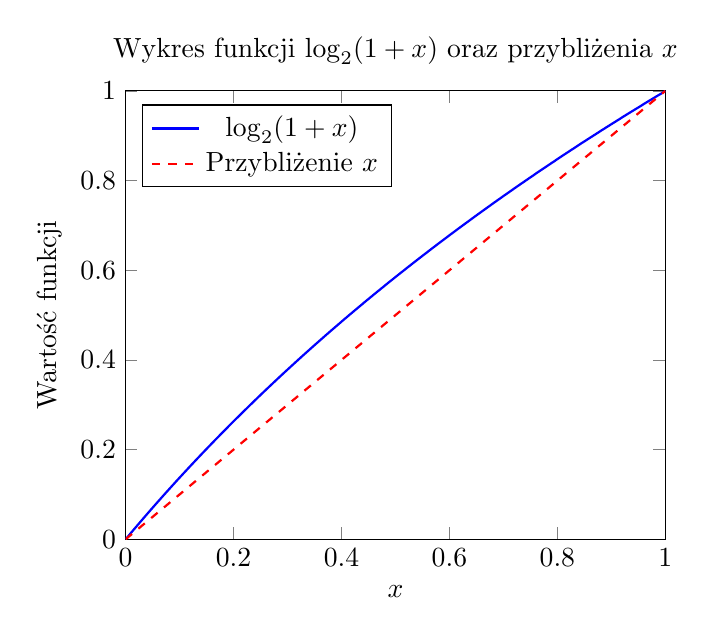
\begin{tikzpicture}
\begin{axis}[
    title={Wykres funkcji $\log_2(1 + x)$ oraz przybliżenia $x$},
    xlabel={$x$},
    ylabel={Wartość funkcji},
    xmin=0, xmax=1,
    ymin=0, ymax=1,
    legend pos=north west,
    grid style=dashed,
]

% Dodajemy krzywe
\addplot[
    domain=0:1,
    samples=400,
    color=blue,
    thick,
]
{log2(1 + x)};
\addlegendentry{$\log_2(1 + x)$}

\addplot[
    domain=0:1,
    samples=400,
    color=red,
    dashed,
    thick,
]
{x};
\addlegendentry{Przybliżenie $x$}

\end{axis}
\end{tikzpicture}
\caption{Porównanie funkcji $\log_2(1 + x)$ i jej przybliżenia $x$.}
\end{figure}

\end{document}
